% Common preamble for PIGMIE patent figures (A4).
% Drawing conventions:
%   - A4 portrait
%   - Sans-serif throughout (Helvetica)
%   - "Fig. N" sentence-case caption near top
%   - Page "N/total" at top centre
%   - Reference numerals outside boxes via leader lines
%   - ALL CAPS labels in component boxes
%   - Reactor uses north-east-lines hatched fill
%   - Scene uses double-line border
%   - Module enclosures use dashed line with internal numeral

\documentclass[a4paper,10pt]{article}
\usepackage[top=2.5cm,bottom=1.0cm,left=2.5cm,right=1.5cm]{geometry}
\usepackage[T1]{fontenc}
\usepackage{helvet}
\renewcommand{\familydefault}{\sfdefault}
\usepackage{amsmath,amssymb,bm}
\usepackage{tikz}
\usetikzlibrary{shapes,shapes.geometric,shapes.misc,arrows.meta,positioning,fit,calc,backgrounds,decorations.pathreplacing,decorations.markings,patterns}
\pagestyle{empty}
\setlength{\parindent}{0pt}

\tikzset{
  % Component box: ALL CAPS label inside, no numeral inside
  cbox/.style={draw, rectangle, minimum height=1.0cm, minimum width=2.4cm,
               align=center, line width=0.5pt, font=\small},
  cbox-tall/.style={cbox, minimum height=1.6cm},
  cbox-wide/.style={cbox, minimum width=3.0cm},
  cbox-narrow/.style={cbox, minimum width=1.8cm, font=\footnotesize},
  % Reactor / physical medium: hatched fill
  reactor/.style={cbox, pattern=north east lines, pattern color=black!70},
  % Scene: double-line border
  scenebox/.style={cbox, double, double distance=1.2pt, line width=0.4pt},
  % Module / sub-module enclosure
  enclosure/.style={draw, rectangle, dashed, line width=0.4pt, inner sep=10pt, rounded corners=2pt},
  enclosure-solid/.style={draw, rectangle, line width=0.5pt, inner sep=10pt, rounded corners=2pt},
  % Arrows
  flowarr/.style={-Latex, line width=0.5pt, font=\scriptsize},
  flowbi/.style={Latex-Latex, line width=0.5pt, font=\scriptsize},
  flowarr-fb/.style={-Latex, line width=0.5pt, dashed, font=\scriptsize},
  % Reference numeral leader-line endpoint and label
  refnum/.style={font=\footnotesize, inner sep=1pt},
  leader/.style={line width=0.4pt, -Latex},
  % Caption banner
  figcap/.style={font=\bfseries\large}
}

% Helper: figure header (page number + Fig. N caption)
\newcommand{\figheader}[3]{%
  % #1 = page number (e.g. "1"), #2 = total pages, #3 = figure label (e.g. "1" or "4A")
  \noindent\hfill\small #1/#2\hfill\null\par
  \vspace{0.2cm}
  \begin{center}\bfseries Fig.\ #3\end{center}
  \vspace{0.2cm}
}


\begin{document}

\figheader{5}{7}{4A}

\begin{center}
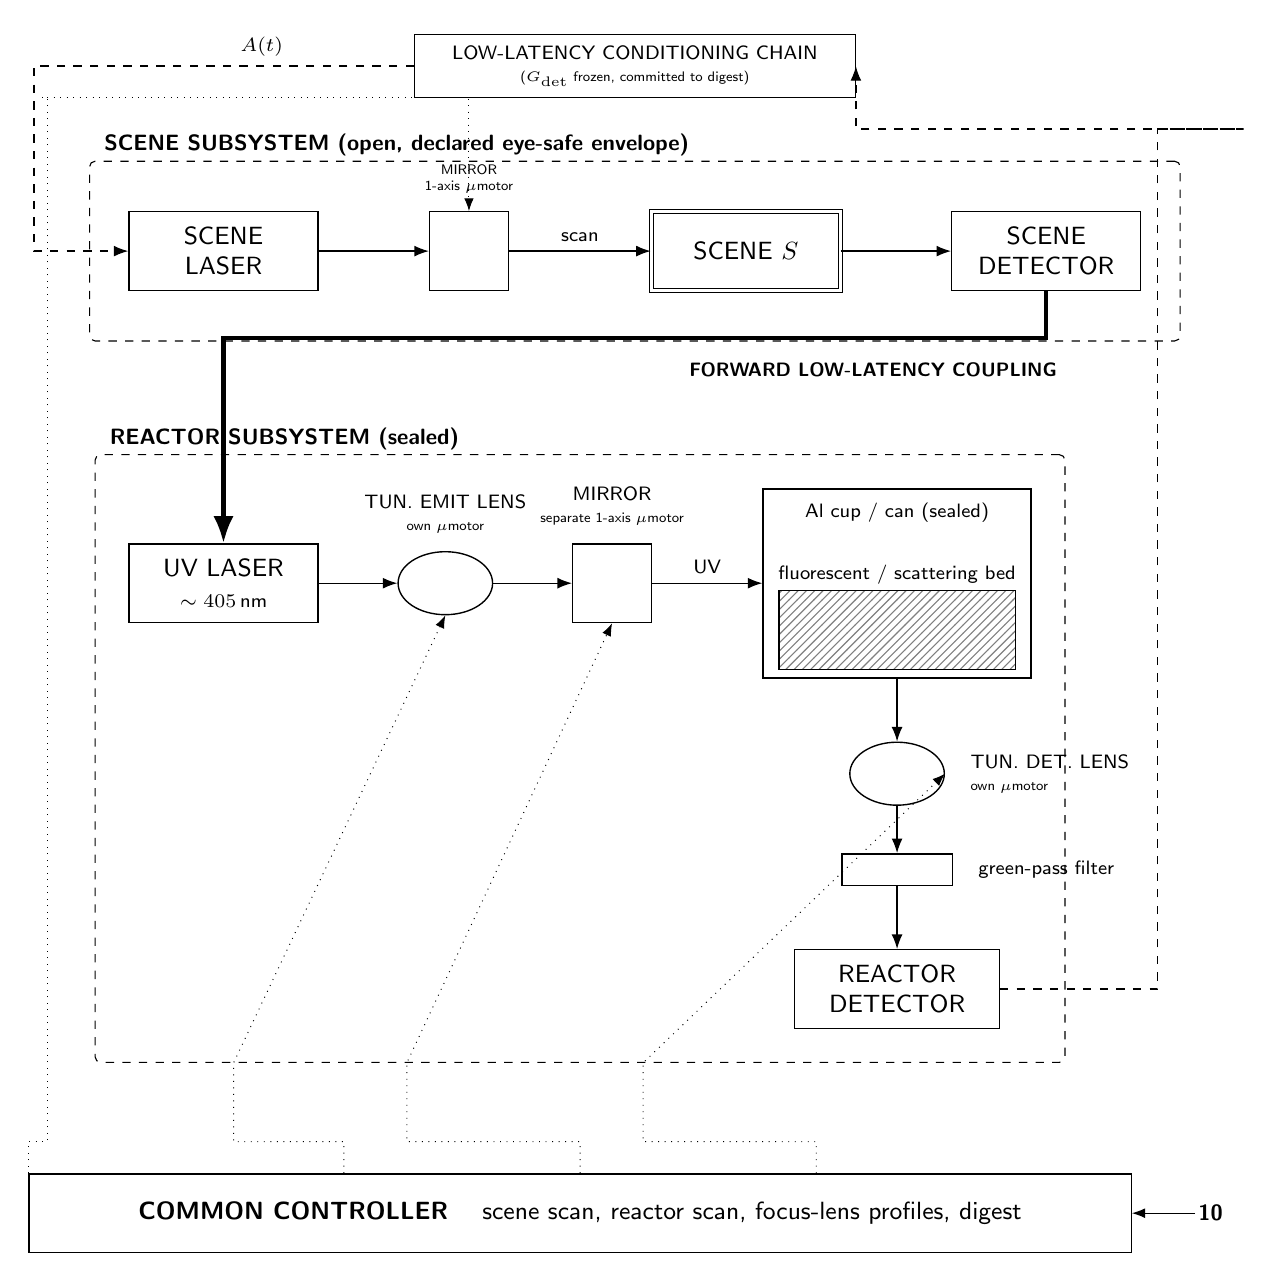
\begin{tikzpicture}[node distance=8mm]

% ============== TOP: SCENE SUBSYSTEM (horizontal row) ==============
\node[cbox, minimum width=2.4cm] (slaser) {SCENE\\LASER};
\node[draw, line width=0.5pt, right=14mm of slaser, minimum width=10mm, minimum height=10mm] (smirror) {};
\node[font=\tiny, above=1mm of smirror, align=center] {MIRROR\\1-axis $\mu$motor};
\node[scenebox, right=18mm of smirror, minimum width=2.4cm] (sscene) {SCENE $S$};
\node[cbox, right=14mm of sscene, minimum width=2.4cm] (sdet) {SCENE\\DETECTOR};

\draw[flowarr] (slaser.east) -- (smirror.west);
\draw[flowarr] (smirror.east) -- node[above, font=\scriptsize] {scan} (sscene.west);
\draw[flowarr] (sscene.east) -- (sdet.west);

\begin{scope}[on background layer]
  \node[enclosure, fit=(slaser)(smirror)(sscene)(sdet), inner sep=14pt, inner ysep=18pt] (sceneenv) {};
\end{scope}
\node[font=\footnotesize\bfseries, anchor=south west] at ($(sceneenv.north west)+(2pt,-2pt)$)
  {SCENE SUBSYSTEM (open, declared eye-safe envelope)};

% ============== MIDDLE: REACTOR SUBSYSTEM ==============
\node[cbox, below=32mm of slaser, minimum width=2.4cm] (uvlaser) {UV LASER\\\scriptsize $\sim 405\,$nm};
\node[draw, ellipse, line width=0.5pt, right=10mm of uvlaser, minimum width=12mm, minimum height=8mm] (femit) {};
\node[font=\scriptsize, above=1mm of femit, align=center] {TUN.\ EMIT LENS\\\tiny own $\mu$motor};
\node[draw, line width=0.5pt, right=10mm of femit, minimum width=10mm, minimum height=10mm] (rmirror) {};
\node[font=\scriptsize, above=1mm of rmirror, align=center] {MIRROR\\\tiny separate 1-axis $\mu$motor};

% Reactor cup with hatched bed
\node[draw, line width=0.6pt, right=14mm of rmirror, minimum width=3.4cm, minimum height=2.4cm] (cup) {};
\node[font=\scriptsize, anchor=north] at ($(cup.north)+(0,-2pt)$) {Al cup / can (sealed)};
\node[draw, line width=0.4pt, pattern=north east lines, pattern color=black!50,
      minimum width=3.0cm, minimum height=1.0cm, anchor=south] at ($(cup.south)+(0,3pt)$) (bed) {};
\node[font=\scriptsize, anchor=south, inner sep=1pt] at ($(bed.north)+(0,1pt)$)
  {fluorescent / scattering bed};

\draw[flowarr] (uvlaser.east) -- (femit.west);
\draw[flowarr] (femit.east) -- (rmirror.west);
\draw[flowarr] (rmirror.east) -- node[above, font=\scriptsize] {UV} (cup.west);

% Detector pickup: chain BELOW the cup, going downward
% Order: cup -> tunable det lens -> green-pass filter -> reactor detector
\node[draw, ellipse, line width=0.5pt, below=8mm of cup, minimum width=12mm, minimum height=8mm] (fdet) {};
\node[font=\scriptsize, right=2mm of fdet, align=left] {TUN.\ DET.\ LENS\\\tiny own $\mu$motor};
\node[draw, line width=0.5pt, below=6mm of fdet, minimum width=14mm, minimum height=4mm] (filter) {};
\node[font=\scriptsize, right=2mm of filter] {green-pass filter};
\node[cbox, below=8mm of filter, minimum width=2.6cm] (rdet) {REACTOR\\DETECTOR};

\draw[flowarr] (cup.south) -- (fdet.north);
\draw[flowarr] (fdet.south) -- (filter.north);
\draw[flowarr] (filter.south) -- (rdet.north);

\begin{scope}[on background layer]
  \node[enclosure, fit=(uvlaser)(femit)(rmirror)(cup)(filter)(fdet)(rdet), inner sep=12pt] (reactenv) {};
\end{scope}
\node[font=\footnotesize\bfseries, anchor=south west] at ($(reactenv.north west)+(2pt,-2pt)$)
  {REACTOR SUBSYSTEM (sealed)};

% ============== CASCADE FORWARD COUPLING (embodiment b) ==============
% Heavy stroke arrow from SCENE DETECTOR -> UV LASER (the reactor emitter).
% This is the load-bearing forward path of the cascade embodiment:
% direct (optical via gain-pumped media, or electrical), low latency.
% Distinguishes embodiment (b) from the parallel-subsystems variant (a).
\draw[-Latex, line width=1.5pt] (sdet.south) -- ++(0,-6mm) -|
  ($(uvlaser.north)+(0,6mm)$) -- (uvlaser.north);
\node[font=\scriptsize\bfseries, align=center, fill=white, inner sep=2pt]
  at ($(sdet.south)+(-22mm,-10mm)$)
  {FORWARD LOW-LATENCY COUPLING};

% A(t) feedback from reactor detector to scene laser amplitude
% Passes through an explicit LOW-LATENCY CONDITIONING CHAIN box.
% Route: rdet -> right -> up over both subsystems -> chain box (top of page) -> down to scene laser.
\node[draw, line width=0.4pt, font=\scriptsize, align=center, inner sep=4pt,
      minimum width=5.6cm, minimum height=8mm] (gchain) at ($(sceneenv.north)+(0,12mm)$)
  {LOW-LATENCY CONDITIONING CHAIN\\\tiny ($G_{\mathrm{det}}$ frozen, committed to digest)};

\draw[flowarr-fb] (rdet.east) -- ++(20mm,0)
  |- ($(sceneenv.north east)+(8mm,4mm)$)
  -| (gchain.east);
\draw[flowarr-fb] (gchain.west) -| node[pos=0.20, above, font=\scriptsize\bfseries] {$A(t)$}
  ($(slaser.west)+(-12mm,0)$)
  -- (slaser.west);

% ============== COMMON CONTROLLER (bottom) ==============
\node[cbox-wide, below=14mm of reactenv.south, minimum width=14cm, minimum height=1.0cm] (ctrl)
  {\textbf{COMMON CONTROLLER} \quad scene scan, reactor scan, focus-lens profiles, digest};

% ============== Controller fan-out: 4 explicit per-servo lines ==============
% Each line targets a distinct servo from the SOUTH side, routed around components
% so no line passes through any other box.

% (i) Scene scan — enter smirror.north from ABOVE the scene subsystem
% Route: ctrl.NW -> left outside both subsystems -> up over scene subsystem top -> right -> down into smirror.north
\draw[line width=0.35pt, dotted, -Latex] (ctrl.north west) -- ++(0,4mm) -|
  ($(reactenv.south west)+(-6mm,0)$) |- ($(sceneenv.north west)+(-6mm,8mm)$)
  -| (smirror.north);

% (ii) Reactor emit-side lens — routed via reactor subsystem south, into femit from below
\draw[line width=0.35pt, dotted, -Latex] ($(ctrl.north)+(-30mm,0)$) -- ++(0,4mm) -|
  ($(reactenv.south)+(-44mm,0)$) -- (femit.south);

% (iii) Reactor steering mirror — routed via reactor subsystem south, into rmirror from below
\draw[line width=0.35pt, dotted, -Latex] (ctrl.north) -- ++(0,4mm) -|
  ($(reactenv.south)+(-22mm,0)$) -- (rmirror.south);

% (iv) Reactor det-side lens — routed via reactor subsystem south, into fdet from below-right
\draw[line width=0.35pt, dotted, -Latex] ($(ctrl.north)+(30mm,0)$) -- ++(0,4mm) -|
  ($(reactenv.south)+(8mm,0)$) -- (fdet.east);

% Controller numeral 10
\node[refnum] at ($(ctrl.east)+(10mm,0)$) (n10) {\textbf{10}};
\draw[leader] (n10.west) -- (ctrl.east);

\end{tikzpicture}
\end{center}

\end{document}
